% Decision Models as Tool Selectors for Coding Agents with Many MCP Tools
% Real MCP catalog (613 / 1,076 tools), opencode and Hermes Agent harnesses.
% Self-contained submission version: compile with `latexmk -pdf coding_agents.tex` in this folder.
% --- preamble (inlined from shared/preamble.tex) ---
\documentclass[11pt]{article}
\usepackage[T1]{fontenc}
\usepackage[utf8]{inputenc}
\usepackage{lmodern}
\usepackage{microtype}
\usepackage[margin=1in]{geometry}
\usepackage{amsmath,amssymb}
\usepackage{booktabs}
\usepackage{tabularx}
\usepackage{multirow}
\usepackage{graphicx}
\usepackage{xcolor}
\usepackage{enumitem}
\usepackage{caption}
\usepackage{subcaption}
\usepackage{fvextra}
\usepackage{tikz}
\usetikzlibrary{positioning,arrows.meta,shapes.geometric,fit,calc}
\usepackage[numbers,sort&compress]{natbib}
\usepackage[colorlinks=true,linkcolor=blue!50!black,citecolor=blue!50!black,urlcolor=blue!50!black]{hyperref}

\setlist{itemsep=2pt,topsep=3pt}
\captionsetup{font=small,labelfont=bf}
\setlength{\emergencystretch}{3em}
\let\oldus\_\renewcommand{\_}{\oldus\discretionary{}{}{}}
\newcommand{\msd}{MSD1}
% --- end preamble ---
\usepackage{longtable}
\usepackage{array}
\usepackage{xurl}

\newcommand{\dmn}{DM\,+\,none}

\title{\textbf{Decision Models as Tool Selectors for Coding Agents with Many MCP Tools}}
\author{Aziz Muminov \and Alexandra Ilina}
\date{November 2026}

\begin{document}
\maketitle

\begin{abstract}
A coding agent connected to many MCP servers must either load every tool definition into its context (about
180k tokens for the 613 tools of twelve popular servers) or find tools through search. Harnesses use different
mechanisms: name lists with keyword search (Claude Code), BM25 (Codex, Anthropic's tool search, Hermes Agent) and
tool groups (GitHub Copilot); Goose offered embedding and LLM routers in 2025 (since removed). We ask whether a
\emph{decision model} (DM), here Microsoft Decision~1 (\texttt{microsoft/microsoft-decision-1} on OpenRouter's
Decisions API), which returns a probability per option for up to 255 options without generating text, is a
better tool selector. We built a test suite from the real tool definitions of 30 MCP servers (613 and 1{,}076
tools) with simulated back ends, 38 coding tasks graded by hidden tests and required writes, and two agent
harnesses (opencode and Hermes Agent). Our main experiment swaps the ranker inside Hermes Agent's tool-search
bridge (BM25, Microsoft Decision~1 with and without a ``none'' option, embeddings, a Claude Code-style ranker,
random) on 38 tasks over 1{,}076 tools, pinned and paired (684 runs). Every ranker, even random, passed 96--100\%
of runs, but ranking showed in tokens: random used 1.57$\times$ the tokens of BM25. The DM rankers and embeddings
used 7--12\% fewer tokens than BM25; only DM with the ``none'' option had a 95\% CI excluding 1 (0.88$\times$,
0.78--0.98), and not after Bonferroni correction for five comparisons. With the DM, agents needed fewer searches
per needed tool (2.7 against 3.4). Offline, a server-then-tool DM hierarchy ranks best (hit@1 0.93 at 613 tools
against 0.48--0.54 for name, BM25 and embedding search and 0.86 for an LLM router). A projection suggests the
DM's per-search fee pays off for agent models costing more than about \$0.03 per run.
\end{abstract}

%=====================================================================
\section{Introduction}\label{sec:intro}
%=====================================================================
Through the Model Context Protocol (MCP)~\citep{mcp}, coding agents read CI logs, error trackers, tickets, chat,
dashboards, clusters and databases, and the LLM must see each tool's definition (name, description, parameter
schema) before calling it. Twelve widely used servers (GitHub, Grafana, Sentry, Atlassian, Linear, Slack, Notion,
Kubernetes, MongoDB, Postgres, Git, Playwright) expose 613 tools whose definitions take about 180k tokens per
request.

Harnesses therefore use \emph{tool search}: definitions stay out of the prompt and the agent finds tools on demand
(\S\ref{sec:background}). Claude Code defers MCP tools, lists only their names, and loads them through a
ToolSearch tool~\citep{claudecode}; Anthropic's API and OpenAI's Codex CLI offer BM25
search~\citep{anthropic2025toolsearch,codexcli}; GitHub Copilot groups tools into ``virtual tools'' that the agent
activates~\citep{copilotvirtualtools}; Goose offered embedding-based and LLM-based tool routers as a preview in
2025 (since removed)~\citep{goose}; Hermes Agent defers MCP tools behind a BM25 search tool~\citep{hermesagent}.
These ranking functions have not been compared on the same tools and tasks.

\emph{Decision models} (DMs) suit this ranking: a DM reads a state and a question with named options and returns
a probability per option in one forward pass, without generating tokens. We use Microsoft Decision~1 (\msd{};
\texttt{microsoft/microsoft-decision-1})~\citep{msd1} through OpenRouter's Decisions API~\citep{openrouterdecisions}.
But a DM accepts at most 255 options, fewer than a realistic catalog, and cannot write arguments.

We ask: \emph{can a DM serve as a coding agent's tool selector, and is it better than the mechanisms harnesses
use?} Our test suite (\S\ref{sec:suite}) uses the real \texttt{tools/list} output of 30 MCP servers (613 tools,
1{,}076 with decoys such as GitLab beside GitHub), simulated back ends, 38 graded tasks (33 in two prompt
versions, plus five), eight selection conditions and two harnesses. In brief (caveats in \S\ref{sec:threats}):
\begin{itemize}
\item \textbf{Main experiment (\S\ref{sec:final}).} Six rankers in Hermes Agent's search bridge, two of them
Microsoft Decision~1 (DM, and \dmn{}, which may answer that no tool fits); 684 paired runs. Every ranker passed
96--100\% of runs. Random ranking used 1.57$\times$ the tokens of BM25, so ranking matters. The DM rankers and
embeddings leaned 7--12\% below BM25; only \dmn{}'s 95\% CI excluded 1 (0.88$\times$, 0.78--0.98), not after
Bonferroni correction (99\% CI 0.75--1.02), and \dmn{} and DM did not differ significantly. The saving comes from
fewer LLM calls and smaller prompts; with the DM, agents needed fewer searches to reach each needed tool.
\item \textbf{Offline (\S\ref{sec:retrieval}).} At 613 tools the DM hierarchy put the right tool first for 93\%
of 120 hand-written queries, against 48--54\% for name, BM25 and embedding search and 86\% for an LLM router
(1{,}076 tools: 88\%, 45--49\%, 82\%), at a third of the router's cost; on agent-written queries the gap is smaller.
\item \textbf{Live, eight mechanisms (\S\ref{sec:opencode}).} With opencode every catalog condition passed
96--100\% of runs, and search cut the largest prompt from about 182k tokens to 12--53k, so pass rate cannot
separate rankers; tokens must be compared, paired.
\end{itemize}

\paragraph{Contributions.} (i)~A test suite for tool selection in coding agents on real MCP tool definitions,
with simulated back ends, graded tasks and an isolated sandbox. (ii)~A Microsoft Decision~1 tool ranker that
passes the 255-option limit by choosing the server first, integrated into a shipped harness's search bridge.
(iii)~A comparison of current mechanisms and the DM, offline and in two agents, with a paired, pinned protocol
for measuring token differences between agent configurations.

%=====================================================================
\section{How harnesses select tools}\label{sec:background}
%=====================================================================
Table~\ref{tab:mechanisms} lists the mechanisms we compare. All but native loading give the agent a search tool
and a way to call what it finds, usually with a short server overview, so it pays for definitions only on
retrieval.

\begin{table}[t]
\centering\footnotesize
\caption{Tool-selection mechanisms and the conditions that reproduce them. Used in: M, main experiment
(\S\ref{sec:final}); R, offline retrieval (\S\ref{sec:retrieval}); O, opencode (\S\ref{sec:opencode}).}
\label{tab:mechanisms}
\setlength{\tabcolsep}{4pt}
\begin{tabularx}{\linewidth}{@{}l >{\raggedright\arraybackslash}p{3.6cm} X l@{}}
\toprule
Condition & Shipped or proposed in & What the agent sees and does & Used in \\
\midrule
none & control & no catalog tools at all & O \\
native & Cursor, Cline, opencode; Claude Code with search off & every tool definition in every request & O \\
cc & Claude Code ToolSearch~\citep{claudecode} & names of all deferred tools; \texttt{select:a,b} by exact name, or keyword search with name matches weighted highest (our approximation; the exact scoring is undocumented) & M R O \\
bm25 & Anthropic tool search~\citep{anthropic2025toolsearch}, Codex CLI~\citep{codexcli}, Hermes~\citep{hermesagent} & Okapi BM25~\citep{robertson2009bm25} over names, descriptions and parameters & M R O \\
groups & GitHub Copilot virtual tools~\citep{copilotvirtualtools} & one \texttt{activate\_<group>} tool per server (servers over 40 tools split); activating loads the group's definitions & O \\
embed & RAG-MCP~\citep{gan2025ragmcp}, Goose (2025, removed)~\citep{goose} & cosine similarity of \texttt{text-embedding-3-small} vectors of query and tool & M R O \\
llm & Goose (2025, removed)~\citep{goose}, AnyTool-style LLM routing~\citep{du2024anytool} & an LLM (DeepSeek V4.1 Flash) reads one line per tool and names the best ones & R O \\
dm & this paper & Microsoft Decision~1 (\texttt{microsoft/microsoft-decision-1}) ranks servers, then tools; \dmn{} adds a ``none'' option (\S\ref{sec:dm}) & M R O \\
random & control & five random tools & M \\
\bottomrule
\end{tabularx}
\end{table}

\paragraph{Hermes's bridge.} Hermes Agent 0.19.0 defers MCP tools once their definitions exceed 10\% of the
context window, as 613 tools do. \texttt{tool\_search} returns compact hits (name and one line),
\texttt{tool\_describe} one full definition, and found tools are called directly with typed arguments. Our main
experiment swaps only the ranker behind \texttt{tool\_search} (Figure~\ref{fig:dmflow}).

%=====================================================================
\section{Decision models as tool selectors}\label{sec:dm}
%=====================================================================
\paragraph{The interface.} A Decisions API request carries a \emph{state} (here the agent's search query) and
named questions; a \texttt{choice} question lists options, each with a free-text description, and returns a
probability per option~\citep{openrouterdecisions}. We describe each tool by its name, the first 300 characters
of its description and its parameter names. The DM in all our experiments is Microsoft Decision~1 (\msd{}),
called as \texttt{microsoft/microsoft-decision-1} on OpenRouter's Decisions API and post-trained from
Qwen3.5-9B~\citep{msd1}; it answered in about half a second in our runs and costs \$0.042 per million input
tokens.

\paragraph{The 255-option limit.} The API rejects \texttt{choice} questions with more than 255 options, and
\msd{} rejects requests beyond about 32k tokens. We compared four ways around the limit:
\begin{itemize}
\item \textbf{Hierarchy} (default): ask which server has the needed tool (12 or 30 options, each described by
the server's purpose), take the most likely servers until they cover 90\% of the probability mass (at most
three), ask which of their tools fits (Linear, the largest server, has 198), and score each tool by
$P(\text{server})\cdot P(\text{tool}\mid\text{server})$.
\item \textbf{Tournament}: split the catalog into chunks of at most 250, keep the top five of each, and decide
among the survivors.
\item \textbf{BM25$\to$DM} and \textbf{embed$\to$DM}: shortlist 100 tools with BM25 or embeddings, then let the
DM choose among them.
\end{itemize}

\paragraph{The ``none'' option.} \dmn{} adds an option ``none of these services'' to the server question and
returns no tools when $P(\text{none})\ge0.4$, otherwise at most five. The threshold was tuned on the offline
benchmark (\S\ref{sec:retrieval}). Figure~\ref{fig:dmflow} shows the hierarchy inside Hermes's bridge.

\begin{figure}[t]
\centering
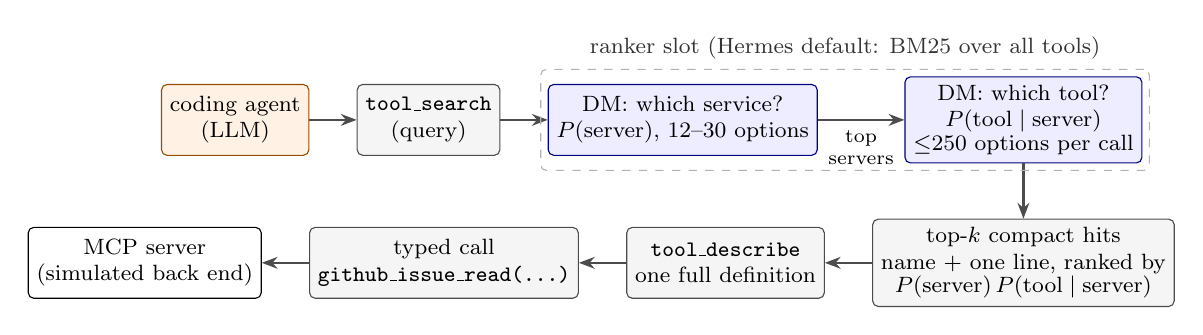
\begin{tikzpicture}[font=\footnotesize, node distance=4mm and 6mm,
  box/.style={draw, rounded corners=2pt, align=center, inner sep=3pt, minimum height=9mm, fill=white},
  dm/.style={box, fill=blue!7, draw=blue!50!black}, llm/.style={box, fill=orange!10, draw=orange!60!black},
  outb/.style={box, fill=gray!8, draw=gray!60!black}, arr/.style={-{Stealth[length=2mm]}, thick, draw=gray!60!black}]
\node[llm] (agent) {coding agent\\ \footnotesize (LLM)};
\node[outb, right=of agent] (search) {\texttt{tool\_search}\\ \footnotesize (query)};
\node[dm, right=of search] (srv) {DM: which service?\\ \footnotesize $P(\text{server})$, 12--30 options};
\node[dm, right=11mm of srv] (tool) {DM: which tool?\\ \footnotesize $P(\text{tool}\mid\text{server})$\\[-1pt] \footnotesize $\le$250 options per call};
\node[outb, below=7mm of tool] (hits) {top-$k$ compact hits\\ \footnotesize name + one line, ranked by\\[-1pt] \footnotesize $P(\text{server})\,P(\text{tool}\mid\text{server})$};
\node[outb, left=of hits] (desc) {\texttt{tool\_describe}\\ \footnotesize one full definition};
\node[outb, left=of desc] (call) {typed call\\ \footnotesize \texttt{github\_issue\_read(\dots)}};
\node[box, left=of call] (svc) {MCP server\\ \footnotesize (simulated back end)};
\draw[arr] (agent) -- (search);
\draw[arr] (search) -- (srv);
\draw[arr] (srv) -- node[below, font=\scriptsize, align=center]{top\\servers} (tool);
\draw[arr] (tool) -- (hits);
\draw[arr] (hits) -- (desc);
\draw[arr] (desc) -- (call);
\draw[arr] (call) -- (svc);
\node[draw=gray!60, dashed, rounded corners=2pt, fit=(srv)(tool), inner sep=2.5pt,
  label={[font=\footnotesize, text=gray!40!black]above:ranker slot (Hermes default: BM25 over all tools)}] {};
\end{tikzpicture}
\caption{Tool selection with a decision model inside Hermes Agent's search bridge. The agent's query goes to the
ranker slot, where the DM first chooses among servers and then among the tools of the most likely servers (at most
250 options per call). The agent receives compact hits, reads one full definition with \texttt{tool\_describe},
and calls the tool directly with typed arguments. In the default harness BM25 fills the same slot; everything
outside the dashed box is identical across conditions.}
\label{fig:dmflow}
\end{figure}

\paragraph{Why the DM selects and does not call.} A DM cannot write arguments, and most tool choices in a coding
session are easy: predicting the next tool of a real session, \msd{} did worse than always choosing the shell,
while always-loaded definitions took most of the first request (App.~\ref{app:session}). The DM belongs in the
catalog: choosing which of hundreds of rarely used tools to show, while the LLM keeps the core tools and writes
every call.

%=====================================================================
\section{Test suite}\label{sec:suite}
%=====================================================================
\paragraph{Real tool catalog.} We started twelve MCP servers as an unprivileged user with dummy credentials and
saved their \texttt{tools/list} responses: names, descriptions and input schemas exactly as published. No tool
was ever executed against a real service. This main catalog has 613 tools from 12 servers, from Linear (198),
Atlassian (98), GitHub (91) and Grafana (81) down to Postgres (1). Eighteen further servers add 463 tools (1{,}076
in all), including natural decoys: GitLab beside GitHub, AWS CloudWatch beside Grafana Loki, AWS EKS beside
Kubernetes (all servers in App.~\ref{app:catalog}).

\paragraph{Simulated back ends.} Each task has a world: rules (tool, argument values to match, response), then
organization-wide facts shared by all tasks; the first matching rule answers. Unmatched reads return what a real
service would for something that does not exist (empty list or not found); unmatched writes succeed and are
recorded for grading. Optionally, arguments are validated against the tool's schema.

\paragraph{Tasks.} Each task is a small Python repository whose fix needs information that lives only in the
services (a failing CI check, a Sentry stack trace, Loki logs, an alert threshold, a crash-looping pod, a Slack
decision, a ticket, a wiki page, a document shape, a schema), reachable only through the catalog since the sandbox
has no network or credentials. Many tasks also require a write (comment on the pull request, resolve the Sentry
issue, move the ticket, reply in the thread, open a pull request).
\begin{itemize}
\item \textbf{v1} (33 tasks): 22 single-service, 3 multi-service, 4 \emph{absent} (the information does not
exist; the right outcome is to stop and leave a \texttt{TODO}), and 4 controls that need no catalog tool. Prompts
often name the service (``check the logs in Loki'').
\item \textbf{v2} (38 tasks, App.~\ref{app:tasks}): the same worlds with \emph{symptom-first} prompts that do
not name the service (``customers stopped getting shipping e-mails''), a shared ``where things live'' handbook in
every README (like an \texttt{AGENTS.md}, naming the company's tools, including legacy GitLab, CloudWatch and
EKS), and five new tasks, four multi-service and three on the extra servers, so that the decoy servers are
sometimes the right answer.
\end{itemize}
The offline retrieval queries and the opencode runs use v1 with the 613-tool catalog; the main experiment uses v2
with all 1{,}076 tools. Every prompt ends with the same escape clause: if the information is not available, do
not guess; leave the code unchanged and add a \texttt{TODO: info not found} comment. In the main experiment
(\S\ref{sec:final}) every prompt also starts, identically in all conditions, with a note standing in for what
real harnesses say in the system prompt about connected MCP servers: ``Note: the company's internal services
(code hosting, CI, error tracking, metrics and logs, incidents and on-call, tickets, docs and runbooks, chat,
clusters, databases) are connected to you as tools. Some tools are loaded on demand: if a tool you need is not
listed, use tool search to find it.''

\paragraph{Grading and validation.} A run passes when the hidden tests pass, every required write was made with the
right arguments, and no destructive call was made (merge, delete, rollout restart, \texttt{kubectl apply},
\dots). Before use, we checked that each task's hidden tests fail on the original repository and pass with the
reference solution, that every tool it names exists, and that the reference calls get non-empty answers (empty for
absent tasks) and satisfy the required writes.

\paragraph{Harnesses.} \emph{opencode}~\citep{opencode} (v1.19.4) runs headless with a shell limited to
\texttt{pytest} and file tools limited to the project; our MCP server implements every condition of
Table~\ref{tab:mechanisms}, returning the top five tools with full definitions and a service overview, with calls
through \texttt{call\_tool(name, arguments)}. \emph{Hermes Agent}~\citep{hermesagent} 0.19.0 uses its own bridge
(\S\ref{sec:background}) over our server's full tool list; we patched its search function to ask our server's
\texttt{/rank} endpoint, so only the ranker differs (Figure~\ref{fig:dmflow}).

\paragraph{Isolation.} Runs execute as an unprivileged user without credentials, reaching only the LLM proxy (which
holds the API key) and the MCP server; each Hermes run also has its own mount namespace, a per-run MCP token hidden
from the agent's shell, and a deny list of probing commands (App.~\ref{app:hardening}).

%=====================================================================
\section{Experiments}\label{sec:experiments}
%=====================================================================
The main experiment asks whether the ranker changes accuracy or tokens in a shipped harness with everything else
fixed; a projection reuses its token counts to ask at which agent-model price the DM's fee pays off. Offline
retrieval removes the agent and asks which ranker puts the right tool first and how to take the DM past 255
options. The opencode runs ask whether the tasks need the catalog and how much context search saves against
loading every tool (Table~\ref{tab:overview}).

\begin{table}[t]
\centering\footnotesize
\caption{Experiments at a glance. Tasks: task set (\S\ref{sec:suite}); conditions as in
Table~\ref{tab:mechanisms}.}
\label{tab:overview}
\setlength{\tabcolsep}{4pt}
\begin{tabularx}{\linewidth}{@{}lll>{\raggedright\arraybackslash}Xlr@{}}
\toprule
Experiment & Harness & Tasks $\times$ tools & Agent LLM & Compared & Runs \\
\midrule
Main (\S\ref{sec:final}) & Hermes Agent 0.19.0 & v2: 38 $\times$ 1{,}076 & DeepSeek V4.1 Flash (pinned) & 6 rankers & 684 \\
Offline retrieval (\S\ref{sec:retrieval}) & none & 120 queries $\times$ 613, 1{,}076 & none (router: DeepSeek) & 8 rankers & -- \\
opencode (\S\ref{sec:opencode}) & opencode 1.19.4 & v1: 33 $\times$ 613 & DeepSeek V4.1 Flash, hy4 & 8 conditions & 528 \\
\bottomrule
\end{tabularx}
\end{table}

\subsection{Main experiment: rankers inside Hermes's search bridge}\label{sec:final}
This experiment tests whether the ranker behind tool search changes accuracy or tokens when everything else in a
shipped harness is fixed. Hermes Agent's bridge (Figure~\ref{fig:dmflow}) lets us swap the ranker alone.

\paragraph{Design.} Everything is fixed except the ranker: Hermes Agent 0.19.0 with the isolation of
\S\ref{sec:suite}; task set v2 with schema validation and the connected-services note; and one LLM, DeepSeek V4.1
Flash~\citep{deepseekv41}, pinned to DeepInfra's fp8 endpoint (temperature 0.6, seed 7). The six rankers are
\emph{BM25} (Hermes as shipped; Codex CLI also uses BM25); \emph{DM} (Microsoft Decision~1, server then tool;
top five); \emph{\dmn{}} (the same with the ``none'' option of \S\ref{sec:dm}); \emph{embeddings}
(\texttt{text-embedding-3-small}, as in RAG-MCP); \emph{Claude Code style (cc)} (all deferred tool names in the
prompt, keyword ranking and \texttt{select:<name>}); and \emph{random} (five random tools, a lower bound). Each
ranker ran every task three times ($6 \times 38 \times 3 = 684$ runs); BM25, DM and random were queued repeat by
repeat with each slot's conditions back to back, \dmn{}, cc and embeddings later in parallel batches.
\emph{Tokens} are all input (uncached and cached) and output tokens summed over a run's LLM calls, as counted by
Hermes; about 95\% are cached input re-read on every turn, which is why token and cost reductions differ
(\S\ref{sec:projection}). We pair runs by (task, repeat) slot. Tables report medians per run; token ratios are
geometric means of per-slot ratios with a task-level bootstrap 95\% CI (10{,}000 resamples); the projection
uses means. We also report pass@1 and pass$^3$ (the task passes in all three repeats).

\paragraph{Conditions not in the main experiment.} Native loading is covered by the opencode runs
(\S\ref{sec:opencode}). We left out the LLM router and groups: no current harness ships an LLM router (Goose
offered one in 2025 and has since removed it), the router cost about three times as much as the DM per query offline
(Table~\ref{tab:retrieval}), and groups load whole servers (29--53k-token prompts in opencode against 12--35k for
ranked search; Table~\ref{tab:opencode}).

\paragraph{Why paired, and why pinned.} In pilot runs (one is in App.~\ref{app:pilot}) the paired log ratio of
tokens between two conditions had a standard deviation of about 0.44, so detecting a 10\% token difference with
80\% power at $\alpha=0.05$ needs about 136 pairs; the design gives 114 per comparison. Unpinned, OpenRouter
routed DeepSeek requests to dozens of endpoints with different quantizations, and the harness sets no
temperature, hence both fixes. A second LLM, Kimi K3.1 Pro, was piloted and dropped for cost and speed.

\paragraph{Grading.} We corrected two rules during the run (the destructive-call rule matched any tool name
containing ``merge'', blocking a required merge-request comment; one hidden test in \texttt{cw\_reports} rejected a
valid fix) and re-graded all runs from saved artefacts (33 of 684 verdicts changed).

\begin{table}[t]
\centering\footnotesize
\caption{Main experiment: Hermes Agent, DeepSeek V4.1 Flash (pinned), task set v2 (38 tasks), 1{,}076 tools,
three repeats, 114 runs per ranker (684 in all, re-graded). Tokens: all input (uncached and cached) and output
tokens of a run, median per run. Ratio: geometric mean of per-slot token ratios against BM25 with a task-level
bootstrap 95\% CI. Fewer: slots (of 114) on which the ranker used fewer tokens than BM25. LLM calls and searches:
mean per run; time: median wall time per run. Bold: best token values. Pass-rate differences amount to at most
four runs and are not significant.}
\label{tab:final}
\setlength{\tabcolsep}{4pt}
\begin{tabular}{@{}lcccccccc@{}}
\toprule
Ranker & pass@1 & pass$^3$ & Tokens & Ratio [95\% CI] & Fewer & LLM calls & Time (s) & Searches \\
\midrule
BM25 (Hermes, Codex) & 0.991 & 37/38 & 558k & -- & -- & 29.0 & 187 & 11.4 \\
\dmn{} & 0.991 & 37/38 & \textbf{459k} & \textbf{0.88} [0.78, 0.98] & \textbf{69} & 27.4 & 196 & 10.1 \\
DM & 0.991 & 37/38 & 480k & 0.93 [0.82, 1.04] & 66 & 27.9 & 173 & 9.7 \\
embeddings & 0.965 & 35/38 & 562k & 0.91 [0.81, 1.03] & 63 & 27.9 & 175 & 11.1 \\
Claude Code style & 0.991 & 37/38 & 576k & 1.02 [0.89, 1.16] & 43 & 23.2 & 144 & 6.0 \\
random & 1.000 & 38/38 & 1{,}051k & 1.57 [1.38, 1.79] & 27 & 34.9 & 271 & 12.8 \\
\bottomrule
\end{tabular}
\end{table}

\begin{figure}[t]
\centering
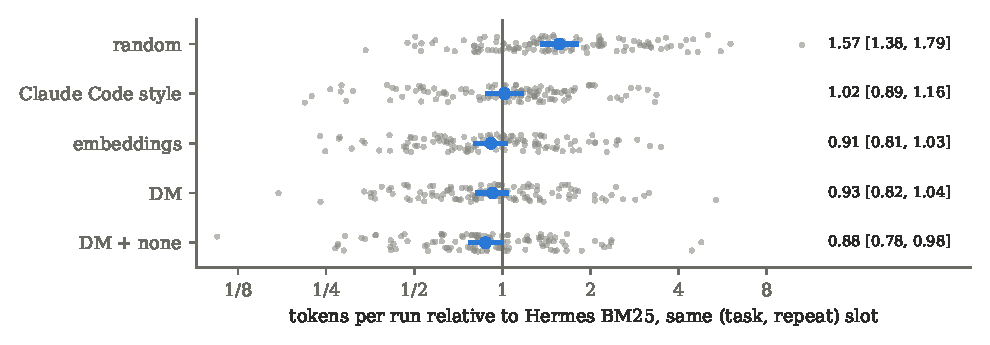
\includegraphics[width=\linewidth]{figures/fig_final.pdf}
\caption{Tokens per run relative to BM25 in the same (task, repeat) slot, 114 slots per ranker. Grey: single
slots; blue: geometric mean with task-level bootstrap 95\% CI (values at right). Single-slot ratios span roughly
0.25--4$\times$, so only paired averages over many slots are informative: random is shifted clearly to the right,
the learned rankers slightly to the left.}
\label{fig:final}
\end{figure}

\paragraph{Accuracy is at ceiling for every ranker, including random.} All six rankers passed 96.5--100\% of runs
and abstained correctly on all 12 absent-task runs (Table~\ref{tab:final}); given five useless tools, an agent
simply searches again. The remaining failures are real: \texttt{kubectl exec} in a production pod in
\texttt{k8s\_crashloop} (destructive; once each under BM25, DM and Claude Code style, twice under embeddings), a
wrong fix in \texttt{cw\_reports} (\dmn{}, embeddings), and unchanged code in \texttt{prom\_threshold}
(embeddings).

\paragraph{Ranking shows up in tokens.} Random ranking cost 1.57$\times$ the tokens of BM25 [1.38, 1.79] and used
fewer tokens on only 27 of 114 slots, so the ranker matters (Figure~\ref{fig:final}). The two Microsoft Decision~1
rankers and embeddings leaned 7--12\% below BM25. \dmn{} was lowest, 0.88$\times$ [0.78, 0.98], with fewer tokens on 69 of
114 slots, and the only ranker whose 95\% CI excludes 1; after Bonferroni correction for the five comparisons with
BM25 (99\% CI 0.75--1.02) it does not, and compared directly with DM it is not significantly different
(0.95$\times$ [0.84, 1.05]). DM (0.93$\times$ [0.82, 1.04]) and embeddings (0.91$\times$ [0.81, 1.03]) had
intervals including 1; embeddings also had the lowest pass rate. The Claude Code-style ranker tied with BM25
(1.02$\times$).

\paragraph{Where the saving comes from.} \dmn{} runs made fewer LLM calls than BM25 runs (0.94$\times$, 27.4
against 29.0) and sent smaller prompts per call (median 19.2k against 21.1k tokens; paired 0.93$\times$ [0.89,
0.97]). With the DM, agents reached each needed tool in fewer searches (Table~\ref{tab:replay}): 2.7 on average
against 3.4 with BM25, and 30\% of needed tools took three or more searches against 46\%; the paired difference
is significant for DM ($-0.71$ searches per needed tool [$-1.13$, $-0.25$], 90 slots) but not for \dmn{}
($-0.25$ [$-0.83$, 0.48]) or embeddings ($-0.13$ [$-0.68$, 0.54]). With BM25 the agent more often had to rephrase
and search again. By task category (few tasks, so only a hint), the ``none'' option helped where the information
does not exist: on absent tasks (4 tasks, 12 slots) \dmn{} used 0.78$\times$ the tokens of BM25 and DM
1.28$\times$, as the agent stopped searching sooner; on multi-service tasks (7 tasks) both used 0.78--0.81$\times$,
on single-service tasks (23) 0.90--0.92$\times$, on controls (4) 0.93--0.97$\times$. The Claude Code-style ranker
made the fewest LLM calls (0.82$\times$ [0.75, 0.90]) and was fastest (0.81$\times$ wall time [0.72, 0.90]),
because agents picked tools from the name list (6.0 searches per run against 11.4), but every prompt carried
1{,}076 names (median 25.8k tokens per call), so its tokens tied with BM25. The DM adds about 0.5\,s per search;
wall time with the DM rankers did not differ significantly from BM25 (\dmn{} 1.04$\times$ [0.90, 1.19], DM
1.03$\times$ [0.94, 1.14]).

\begin{table}[t]
\centering\footnotesize
\caption{Search accuracy and effort in the main run (4{,}785 searches from the 408 runs of four rankers). Hit: the five results contain a tool of the oracle label, over the
2{,}862 searches made while a needed tool was missing. Live: results agents received; replay: every query sent
to every ranker; by writer: range over the rankers under which the queries were written. Searches per needed
tool: searches made while working towards each needed tool (228 per ranker), mean and share needing three or
more. ``None'': \dmn{}'s empty answers among its 1{,}147 live searches, the 2{,}862 replayed queries, and the 879
searches from tasks that need no tool. Bold: best.}
\label{tab:replay}
\setlength{\tabcolsep}{5pt}
\begin{tabular}{@{}lcccccc@{}}
\toprule
& \multicolumn{3}{c}{Hit} & \multicolumn{2}{c}{Searches per needed tool} & \\
\cmidrule(lr){2-4}\cmidrule(lr){5-6}
Ranker & live & replay & by writer & mean & $\ge$3 & ``None'' (live / replay / no-tool) \\
\midrule
BM25 (Hermes) & 0.23 & 0.24 & 0.21--0.25 & 3.43 & 46\% & -- \\
DM & 0.27 & \textbf{0.29} & 0.27--0.30 & \textbf{2.73} & \textbf{30\%} & -- \\
\dmn{} & \textbf{0.28} & 0.28 & 0.27--0.29 & 3.14 & 32\% & 5.6\% / 4.1\% / 9\% \\
embeddings & 0.25 & 0.24 & 0.21--0.25 & 3.09 & 41\% & -- \\
\bottomrule
\end{tabular}
\end{table}

\paragraph{Search accuracy in the live runs.} We gave every search an oracle label: the needed-tool group the agent
was working towards, from the task's list of needs and the agent's successful calls so far. Whichever ranker's
agent wrote the queries, the DMs returned a tool of that group more often than BM25 and embeddings
(Table~\ref{tab:replay}; DM right and BM25 wrong on 228 replayed queries, the reverse on 84), consistent with the
fewer searches per needed tool. Rates are low because many searches are exploratory (``list all available
services'', guesses at services the company does not use): every ranker missed 1{,}890 queries. The live ``none''
answers of \dmn{} we sampled asked for services absent from the catalog (AWS ECS, Google Drive, a Datadog-like
APM).

\subsection{Projection: cost with other agent models}\label{sec:projection}
\emph{This is an analysis of the main run, not a new measurement}: at which agent-model price is the DM's fee
repaid by the tokens it saves? We take the mean token mix per run over all 114 runs of each ranker: BM25 used
34.6k uncached input, 754.5k cached input and 11.6k output tokens (output includes reasoning), \dmn{} 33.3k,
659.7k and 11.1k. The DM's fee, as billed in the run, was \$0.0002 per search, \$0.0020 per run at 10.1
searches. We price both mixes at each model's OpenRouter list price on 5 November 2026 and add the fee to the DM
column (Table~\ref{tab:projection}). This assumes a frontier agent would produce a similar token mix and
reduction; stronger models may instead search less or write better BM25 queries. Since the token reduction itself
is not significant after correction for multiple comparisons, the projection is indicative.

\begin{table}[t]
\centering\small
\caption{\emph{Projected} LLM cost per run with BM25 and with \dmn{} in the bridge (including the DM fee of
\$0.0020 per run), if each model used the mean token mix measured with DeepSeek V4.1 Flash in the main run (114
runs each). Prices: OpenRouter list prices on 5 November 2026, \$ per million tokens (input / cached input /
output). Saving per 1{,}000 runs is BM25 minus DM; negative means the DM costs more. $^{a}$Gemini 4 Argon has the
same list prices as Claude Sonnet 5.5 and GPT-6.1 Sol, and hence the same projection.}
\label{tab:projection}
\setlength{\tabcolsep}{3.5pt}\footnotesize
\begin{tabular}{@{}lcccrr@{}}
\toprule
Agent model & Price (in / cached / out) & BM25 \$/run & DM \$/run & Change & Saving/1k runs \\
\midrule
DeepSeek V4.1 Flash (measured) & 0.15 / 0.003 / 0.60 & 0.0144 & 0.0157 & +9\% & $-$\$1.3 \\
Claude Haiku 5.5 & 0.10 / 0.01 / 0.50 & 0.0168 & 0.0175 & +4\% & $-$\$0.7 \\
Claude Sonnet 5.5$^{a}$ & 2.00 / 0.10 / 10.00 & 0.261 & 0.246 & $-$6\% & \$15 \\
Kimi K3.1 Pro & 2.00 / 0.20 / 10.00 & 0.336 & 0.312 & $-$7\% & \$24 \\
GPT-6.1 Sol$^{a}$ & 2.00 / 0.10 / 10.00 & 0.261 & 0.246 & $-$6\% & \$15 \\
Claude Fable 5.1 & 10.00 / 0.25 / 50.00 & 1.114 & 1.057 & $-$5\% & \$58 \\
\bottomrule
\end{tabular}
\end{table}

\paragraph{The fee is fixed; the saving scales with the agent's price.} At these prices the \dmn{} mix costs
5--8\% less than BM25's before the fee, less than the token reduction because cached input, which fell most
(13\%), is cheap and output fell only 4\%. The fee equals this saving at an agent-LLM cost of \$0.026--0.038 per
run, depending on the model's price ratios, so break-even lies at about \$0.03. Below it, as with the two
inexpensive models, the DM makes a run 4--9\% more expensive; with the mid-range and frontier models, 5--7\%
cheaper (\$15--58 per thousand runs). The fee could be lowered by returning exact tool names found in the query
without a DM call, caching repeated queries, or answering from the server step alone when the DM is confident.

\subsection{Why the DM ranks well: offline retrieval}\label{sec:retrieval}
Offline retrieval removes the agent, so that ranking quality can be measured on fixed queries without agent
noise: it tests which ranker puts the right tool on top, and which of the four strategies of \S\ref{sec:dm} takes
the DM past 255 options. We wrote two queries for each needed step of the v1 tasks, one in natural language and
one as keywords (120 in all), and counted a hit when the top $k$ contained any acceptable tool for that step, at
613 and 1{,}076 tools; the LLM router uses DeepSeek V4.1 Flash (Table~\ref{tab:retrieval}; plotted in
App.~\ref{app:figures}).

\begin{table}[t]
\centering\small
\caption{Offline retrieval on 120 hand-written queries. Hit@$k$: a right tool is among the top $k$. Cost per
1{,}000 queries and median latency of the selecting call at 613 tools; name, BM25 and embedding search run
locally (embedding cost is negligible). Bold: best value per accuracy column.}
\label{tab:retrieval}
\setlength{\tabcolsep}{4.5pt}
\begin{tabular}{@{}lccccccc@{}}
\toprule
& \multicolumn{3}{c}{613 tools} & \multicolumn{2}{c}{1{,}076 tools} & & \\
\cmidrule(lr){2-4}\cmidrule(lr){5-6}
Mechanism & hit@1 & hit@5 & MRR & hit@1 & hit@5 & \$/1k queries & latency (s) \\
\midrule
Claude Code style (cc) & 0.48 & 0.71 & 0.56 & 0.45 & 0.65 & 0 & 0.01 \\
BM25 & 0.54 & 0.75 & 0.62 & 0.49 & 0.76 & 0 & $<$0.01 \\
embeddings & 0.51 & 0.80 & 0.61 & 0.47 & 0.75 & $\approx$0 & 0.67 \\
LLM router & 0.86 & \textbf{0.98} & 0.92 & 0.82 & \textbf{0.98} & 0.44 & 1.31 \\
\midrule
DM hierarchy & \textbf{0.93} & 0.97 & \textbf{0.95} & \textbf{0.88} & 0.97 & 0.15 & 0.54 \\
DM tournament & 0.90 & \textbf{0.98} & 0.94 & 0.86 & \textbf{0.98} & 1.13 & 1.60 \\
BM25$\to$DM & 0.87 & \textbf{0.98} & 0.91 & 0.80 & 0.96 & 0.18 & 0.33 \\
embed$\to$DM & 0.88 & \textbf{0.98} & 0.93 & 0.80 & \textbf{0.98} & 0.18 & 0.99 \\
\bottomrule
\end{tabular}
\end{table}

\paragraph{The DM ranks best; lexical and embedding searches rank worst.} At 613 tools the Microsoft Decision~1
hierarchy put a right tool first for 93\% of queries, the Claude Code-style, BM25 and embedding mechanisms
48--54\%, the LLM router 86\%; learned rankers reached hit@5 of 0.97--0.98, the others 0.71--0.80. The weak
embedding results agree with ToolRet, where general-purpose retrievers do poorly on tool
retrieval~\citep{shi2025toolret}. The DM hierarchy cost \$0.15 per thousand queries, a third of the router's
cost, at under half its latency. On 183 queries written by agents in our live runs the DM's lead is smaller
(App.~\ref{app:agentqueries}).

\paragraph{Choosing the server first is the right way past 255 options.} The hierarchy was the most accurate
strategy at hit@1 and the cheapest. The tournament matched its hit@5 at seven times the cost, since it queries the
DM for every chunk; BM25 or embedding shortlists were as cheap but lost 5--6 points at hit@1 when the shortlist
dropped the right tool. Most needs also lie within one server.

\paragraph{Decoy servers cost every mechanism a little.} Adding 463 tools, including GitLab, CloudWatch and EKS
beside GitHub, Loki and Kubernetes, lowered hit@1 by 3--6 points for every mechanism and left the order unchanged
(DM 0.88, LLM router 0.82, BM25 0.49).

\subsection{Eight mechanisms in a live agent: opencode}\label{sec:opencode}
This experiment checks the premises of the main one in a second harness: that the tasks need the catalog, and how
much context search saves against loading every definition (native), which the main experiment does not include.
Each of the 33 v1 tasks ran under eight conditions (Table~\ref{tab:mechanisms}, including \emph{none}, no catalog)
with two LLMs, DeepSeek V4.1 Flash and Tencent hy4, a second inexpensive model used only here, twice per task and
model (528 runs, 613 tools; Table~\ref{tab:opencode}; plotted in App.~\ref{app:figures}).

\begin{table}[t]
\centering\small
\caption{opencode on task set v1, 613 tools (two repeats per task). Pass: runs passed on the 25 tasks that need
a catalog tool. Largest prompt: median over those runs. Cost: mean LLM cost per run over all 33 tasks, excluding
the selector (LLM router: \$0.0011/\$0.0031 per run; DM: \$0.0003/\$0.0010). Bold: best pass rate and smallest
largest prompt among conditions with catalog access (\emph{none} has no catalog and passes no tool task).}
\label{tab:opencode}
\setlength{\tabcolsep}{4.5pt}
\begin{tabular}{@{}lcccccc@{}}
\toprule
& \multicolumn{3}{c}{DeepSeek V4.1 Flash} & \multicolumn{3}{c}{Tencent hy4} \\
\cmidrule(lr){2-4}\cmidrule(lr){5-7}
Condition & Pass & Largest prompt & \$/run & Pass & Largest prompt & \$/run \\
\midrule
none & 0/25 & 9.6k & 0.0110 & 0/25 & 15.4k & 0.0154 \\
native & \textbf{25/25} & 181.9k & 0.0722 & \textbf{25/25} & 188.5k & 0.1039 \\
cc & \textbf{25/25} & 16.2k & 0.0089 & \textbf{25/25} & \textbf{32.0k} & 0.0375 \\
bm25 & \textbf{25/25} & 13.4k & 0.0093 & \textbf{25/25} & 33.6k & 0.0417 \\
groups & \textbf{25/25} & 29.0k & 0.0179 & 24/25 & 52.7k & 0.0562 \\
embed & \textbf{25/25} & 13.3k & 0.0090 & 23/25 & 49.0k & 0.0514 \\
llm & \textbf{25/25} & \textbf{11.7k} & 0.0076 & \textbf{25/25} & 32.6k & 0.0419 \\
dm & \textbf{25/25} & 14.0k & 0.0082 & \textbf{25/25} & 34.6k & 0.0470 \\
\bottomrule
\end{tabular}
\end{table}

\paragraph{The tasks need the catalog, and every mechanism provides it.} Without a catalog no tool task passed (0
of 50); with one, every condition passed 96--100\% (native, cc, bm25, llm, dm 50 of 50; groups 49; embed 48). All
conditions abstained on the four absent tasks (8 of 8 runs each), and no control run made a catalog call. The three
failures were hy4 runs: twice (groups, embed) the agent also restarted a production Kubernetes deployment unasked
(destructive), and once (embed) it stopped searching before finding the ticket's specification.

\paragraph{Search removes most of the context.} Loading every definition made the largest prompt about 182--189k
tokens; with ranked search it was 12--16k (DeepSeek) and 32--35k (hy4), and 29--53k with groups, whose activation
loads a whole server: 5--16$\times$ less. The cost per run fell from \$0.072 to \$0.008--0.009 for DeepSeek and
from \$0.104 to \$0.038--0.047 for hy4. Differences among ranked searches are within run-to-run noise.

\paragraph{Runs use few tools.} The median catalog run used 4 distinct catalog tools in about 10 calls, almost
always from one server; 23 of the 25 v1 tool tasks need only one server. Choosing the server is most of the
problem, which suits the DM hierarchy but is also easy for any mechanism with a service overview; hence task set v2
and the larger catalog in the main experiment.

%=====================================================================
\section{Threats to validity and lessons}\label{sec:threats}
%=====================================================================
\paragraph{Ceiling, power and multiple comparisons.} Pass rates were at ceiling on v1 and, despite the harder v2
tasks, in the main experiment (96--100\% for every ranker, including random), so we rank by tokens, which are
noisy. With 114 pairs per comparison the main experiment is slightly short of the roughly 136 needed to detect a
10\% token difference. Only random's difference from BM25 survives correction for the five comparisons; the
7--12\% reductions of the learned rankers are a consistent lean, not an established effect.

\paragraph{Scheduling.} BM25, DM and random were queued back to back within each slot; \dmn{}, Claude Code style
and embeddings ran later in parallel batches on the same pinned endpoint. Time-varying provider behaviour (load,
caching, latency) could therefore affect comparisons involving the later three, including \dmn{} against BM25.

\paragraph{Simulated answers.} Real services return longer, messier results, which would raise token counts and could
change how agents search; empty results for unmatched reads may make absent tasks easier to recognize.

\paragraph{The connected-services note.} The note that starts every prompt of the main experiment
(\S\ref{sec:suite}) stands in for what real harnesses say in the system prompt (agents not told what exists may
never search; App.~\ref{app:synthetic}), but it may raise search rates above those of an unprompted agent.

\paragraph{Approximated and omitted mechanisms.} We reimplemented Claude Code's ToolSearch, Copilot's virtual
tools and Goose's routers from their documentation; only Hermes's bridge is shipped code, and our cc scoring in
particular is an approximation. opencode conditions return full definitions and route calls through
\texttt{call\_tool}, Hermes returns compact hits and typed calls, so we compare rankers only within one harness.
The LLM router and groups were tested offline and in opencode but not in the main experiment
(\S\ref{sec:final}).

\paragraph{Query distribution and scale.} Hand-written queries overstate the DM's offline advantage
(App.~\ref{app:agentqueries}). The live results rest on two inexpensive LLMs and one DM, the main experiment on
one LLM.

%=====================================================================
\section{Related work}\label{sec:related}
%=====================================================================
\paragraph{Tool retrieval for large catalogs.} Retrieving tools before generation is the standard answer to large
catalogs~\citep{qin2023toolllm,oats2026}. AnyTool~\citep{du2024anytool} selected among over 16{,}000 APIs with a
hierarchy of LLM agents, category first and tool second; MCP-Zero~\citep{fei2025mcpzero} brings the same
server-then-tool idea to MCP, letting the agent request tools by describing what it needs. Our DM applies this
hierarchy with a decision model instead of an LLM. RAG-MCP~\citep{gan2025ragmcp} retrieves MCP tool descriptions
with embeddings to reduce prompt bloat, and \citet{mudunuri2026semantic} select among 121 tools from five MCP
servers with embeddings, reporting retrieval accuracy and token reduction but no agent task runs. ToolRet finds
that embedding retrievers strong on general benchmarks do poorly on tool retrieval (best nDCG@10
33.8)~\citep{shi2025toolret}, and \citet{selection2026retrieval} find that selecting a tool is largely retrieval.
Agent skills~\citep{anthropic2025skills} apply progressive disclosure to instructions, keeping a one-line summary
in context and loading the body on demand; our service overviews and the v2 handbook play this role for the
catalog. We compare such ideas with shipped mechanisms inside unmodified agents.

\paragraph{MCP benchmarks.} LiveMCPBench~\citep{mo2025livemcpbench} evaluates agents navigating many real MCP
servers, MCPMark~\citep{wu2025mcpmark} stress-tests realistic MCP use with verifiable tasks, and
MCP-Atlas~\citep{mcpatlas2026} and Toolathlon~\citep{toolathlon2025} score task completion with real tools. They
measure end-to-end success; we fix the agent, vary only the selection mechanism, and simulate back ends so runs
are reproducible and writes can be graded safely.

\paragraph{Vendor reports.} Stacklok compared its MCP Optimizer with Anthropic's tool search tool on 2{,}792 tools
and reported much higher selection accuracy for its hybrid retrieval~\citep{stacklok2025optimizer}; Arcade tested
Anthropic's tool search on about 4{,}000 tools~\citep{arcade2025toolsearch}. Both measure selection accuracy, not
task completion, and neither reports token costs per task.

\paragraph{Decision models.} The Artificial Analysis Decision Index~\citep{aa2026decisionindex} and an analysis of
it~\citep{olson2026decision} compare DMs with LLMs on standalone decisions, including tool calling; we place a DM
inside agents as the tool-search ranker.

%=====================================================================
\section{Conclusion}\label{sec:conclusion}
%=====================================================================
A decision model can serve as a coding agent's tool selector. On real MCP tool definitions, Microsoft Decision~1
ranks tools more accurately than the lexical and embedding searches current harnesses use and more cheaply than
an LLM router, and asking for the server first takes it past its 255-option limit. In live agents, however, every
search mechanism reaches ceiling pass rates, and agents' own queries narrow the ranking advantage. Inside Hermes
Agent's bridge the robust result is that ranking matters: random ranking cost 57\% more tokens than BM25. The
Microsoft Decision~1 rankers and embeddings leaned 7--12\% below BM25, with fewer LLM calls, smaller prompts and,
for the DM, fewer searches per needed tool; only the variant with a ``none'' option had a 95\% CI excluding 1
(0.88$\times$, 0.78--0.98), and not after correction for multiple comparisons. If a reduction of this size holds
for other agent models, the DM would make runs 5--7\% cheaper for mid-range and frontier models and 4--9\% more
expensive for inexpensive ones such as the model we measured (\S\ref{sec:projection}). Confirming it needs more
paired slots and conditions run in the same schedule.

\paragraph{Reproducibility.} We will release the tool harvester, catalog snapshots, simulator, the 38 tasks (in
both prompt versions) with hidden tests and reference solutions, the MCP server with all conditions, the Hermes
patch, the sandbox setup, all run records, and the analysis and figure scripts.

\bibliographystyle{plainnat}
\bibliography{references}

\appendix
%=====================================================================
\section{Harness hardening}\label{app:hardening}
%=====================================================================
The setup of \S\ref{sec:suite} is the result of fixes made during development; runs made before them are not
reported. In order:
\begin{itemize}
\item Agents run as an unprivileged user with an empty environment and no credentials; experiment files are
readable only by root and the API key is held by a local proxy that admits only the experiment models
(harness-level permissions alone let an agent read hidden tests through absolute paths).
\item Each Hermes run gets its own mount namespace: a private work directory, home directory and \texttt{/tmp},
so runs cannot see each other's files or leftovers.
\item The MCP server accepts only requests carrying a per-run token that the agent's shell cannot read, so the
shell cannot list the catalog or query the ranker directly.
\item Hermes's \texttt{approvals.deny} list blocks probing commands (\texttt{curl}, \texttt{wget}, \texttt{ps},
\texttt{ss}, \texttt{netstat}, \texttt{nmap}, \texttt{lsof}, \texttt{/proc}, \texttt{localhost}, \texttt{find /}).
\item Rankers are compared inside Hermes's own bridge (compact hits, \texttt{tool\_describe}, typed calls) rather
than through a separate MCP-side search with a generic \texttt{call\_tool}, so that only the ranking differs.
\item The provider and sampling are pinned (DeepInfra fp8, temperature 0.6, seed 7).
\end{itemize}

%=====================================================================
\section{Next-tool prediction in a real session}\label{app:session}
%=====================================================================
This experiment motivates using the DM as a selector rather than as the caller (\S\ref{sec:dm}). We took the 395
tool decisions of one real coding session and asked each model to predict the next tool among the 38 available.
\msd{} reached accuracy 0.49 (TypeSafe Jev~\citep{typesafejev}: 0.60), below ``always the shell'' at 0.75,
although the DMs' top five contained the right tool 94--96\% of the time. In that session 51 always-loaded tool
definitions took about 59k tokens, 93\% of the first request and 16\% of all context tokens read.

%=====================================================================
\section{Offline retrieval on agent-written queries}\label{app:agentqueries}
%=====================================================================
This experiment checks whether the offline ranking of \S\ref{sec:retrieval} carries over to the queries agents
actually write. We took 183 queries from the searches in our live runs, mostly keyword lists and tool-name
fragments, labelled each with the needed tool the agent was working towards, and ran them through the same
mechanisms. The DM still led at hit@1 (0.60 against 0.45 for BM25) but barely at hit@5 (0.70 against 0.66).
Keyword-style queries suit lexical search, and agents compensate for a weak first query by searching again, so
offline ranking quality translates only partly into agent behaviour.

%=====================================================================
\section{Hermes pilot}\label{app:pilot}
%=====================================================================
Before the main experiment we ran Hermes Agent with BM25 and DM on 12 v1 tasks with two repeats and 613 tools
(24 paired slots), analysed as in \S\ref{sec:final}. It pointed the same way: DM used 0.88$\times$ the tokens
of BM25 (95\% CI 0.77--1.02).

%=====================================================================
\section{Figures for the supporting experiments}\label{app:figures}
%=====================================================================
Figures~\ref{fig:retrieval} and~\ref{fig:opencode} plot Tables~\ref{tab:retrieval} and~\ref{tab:opencode}.

\begin{figure}[ht]
\centering
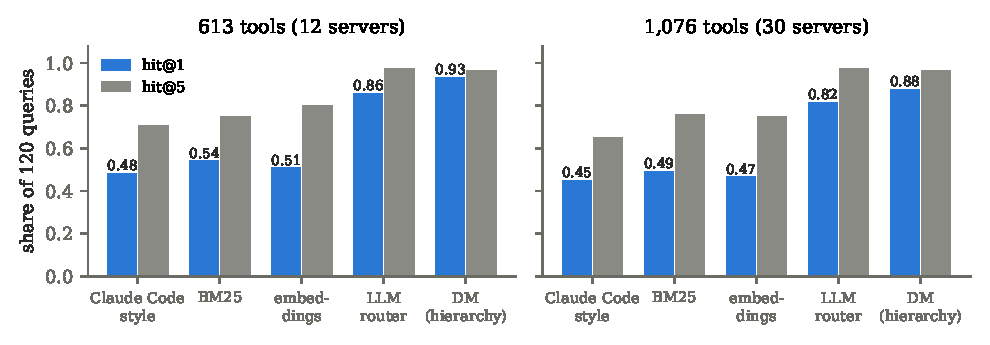
\includegraphics[width=\linewidth]{figures/fig_retrieval_real.pdf}
\caption{Offline retrieval, hit@1 (labelled) and hit@5, on the main and the extended catalog.}
\label{fig:retrieval}
\end{figure}

\begin{figure}[ht]
\centering
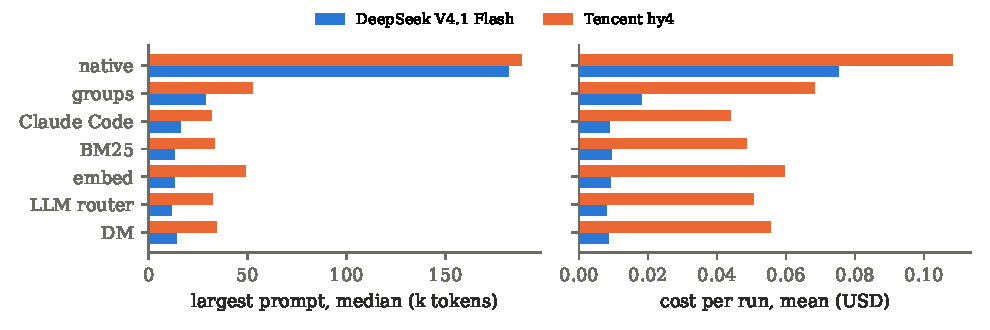
\includegraphics[width=\linewidth]{figures/fig_opencode_real.pdf}
\caption{opencode, task set v1, 613 tools: median largest prompt on the 25 tool tasks and mean cost per run,
by condition and LLM.}
\label{fig:opencode}
\end{figure}

%=====================================================================
\section{The earlier synthetic pilot}\label{app:synthetic}
%=====================================================================
An earlier version of this study used a fictional company's catalog of 100 and 300 synthetic tools (about 610
tokens each) with opencode, and compared loading all tools, a DM-backed \texttt{find\_tool}/\texttt{call\_tool}
pair with and without a service list, and tools preselected from the task prompt. It showed the same pattern as
the real-catalog runs: search matched native loading at a fraction of the context, and an agent without a list of
the services sometimes never searched. We replaced it because its templated descriptions were more uniform and
easier to rank than real ones, its tasks were at ceiling, and its tools resembled no real server, so it could not
compare the mechanisms that harnesses ship. Its code and results remain in the repository.

\clearpage
%=====================================================================
\section{Tool catalog and task set v2}\label{app:catalog}\label{app:tasks}
%=====================================================================
{\centering\footnotesize
\captionof{table}{The real tool catalog: tools per MCP server, from each server's own \texttt{tools/list}.}
\label{tab:catalog}
\setlength{\tabcolsep}{3.5pt}
\begin{tabularx}{\linewidth}{@{}l X r@{}}
\toprule
Catalog & Servers (tools) & Tools \\
\midrule
main & Linear (198), Atlassian (98), GitHub (91), Grafana (81), Git (28), MongoDB (27), Playwright (25), Notion (24),
Kubernetes (23), Sentry (9), Slack (8), Postgres (1) & 613 \\
extra & GitLab (127), monday (84), Salesforce (74), Heroku (33), HubSpot (21), AWS CloudWatch (19), AWS EKS (16),
Airtable (16), Filesystem (14), CircleCI (13), Browserbase (9), Memory (9), Netlify (9), Terraform (9),
Elasticsearch (4), ClickHouse (3), Figma (2), Docker (1) & +463 \\
\midrule
all & 30 servers & 1{,}076 \\
\bottomrule
\end{tabularx}
\par}
\bigskip
{\small
\begin{longtable}{@{}>{\raggedright\arraybackslash}p{1.4cm}>{\raggedright\arraybackslash}p{2.6cm}>{\raggedright\arraybackslash}p{7.1cm}>{\raggedright\arraybackslash}p{2.4cm}@{}}
\caption{Task set v2 (38 tasks). Prompts are shortened to their first sentence and shown without the escape clause. Services: the servers of the needed tools, in order; $+w$: number of required writes; $\star$: new in v2.}\label{tab:tasks_v2}\\
\toprule Category & Task & Prompt (first sentence) & Services \\ \midrule\endfirsthead
\toprule Category & Task & Prompt (first sentence) & Services \\ \midrule\endhead
control & \texttt{c\_chunk} & chunk in batching/chunk.py drops the last partial chunk. & -- \\
control & \texttt{c\_dedupe} & dedupe in collections\_util/dedupe.py loses the original order. & -- \\
control & \texttt{c\_duration} & parse\_duration in timeutil/duration.py only understands hours. & -- \\
control & \texttt{c\_leap} & is\_leap in calendar\_util/leap.py is wrong for some years. & -- \\
single & \texttt{confluence\_limits} & Our public API rate limits changed. & atlassian \\
single & \texttt{eks\_importer} $\star$ & The data team's nightly batch-importer job has failed three nights in a row. & aws\_eks \\
single & \texttt{gh\_ci\_fail} & Pull request \#214 in acme/payments can't be merged because a check is red. & github $+1w$ \\
single & \texttt{gh\_codesearch} & SUPPORTED\_CURRENCIES in shop/currencies.py has drifted from the company-wide canonical list, which lives in another repository. & github \\
single & \texttt{gh\_dependabot} & Security says acme/payments has dependencies with known vulnerabilities. & github \\
single & \texttt{gh\_issue} & Please implement acme/payments\#301. & github \\
single & \texttt{gh\_open\_pr} & Pagination in acme/catalog is broken (see \#57). & github $+2w$ \\
single & \texttt{gh\_release} & We are behind on the ledger API. & github \\
single & \texttt{gh\_review} & There is reviewer feedback waiting on pull request \#88 in acme/ledger. & github $+1w$ \\
single & \texttt{grafana\_incident} & We are in the middle of an incident about checkout timeouts and the responders agreed on a mitigation. & grafana $+1w$ \\
single & \texttt{jira\_impl} & Pick up PAY-412: implement it, then move it to review. & atlassian $+1w$ \\
single & \texttt{k8s\_crashloop} & ledger-worker keeps restarting in production (namespace ledger) since the last config change. & kubernetes \\
single & \texttt{k8s\_oom} & report-builder (namespace reports) keeps dying in production. & kubernetes \\
single & \texttt{linear\_bug} & Fix ENG-77 and move it to In Review. & linear $+1w$ \\
single & \texttt{loki\_errors} & Customers stopped getting shipping e-mails at around 06:00 UTC today; the notifier service is the suspect. & grafana \\
single & \texttt{mongo\_shape} & The nightly export has started crashing on recent orders. & mongodb \\
single & \texttt{notion\_runbook} & We are rotating the webhook signing keys. & notion \\
single & \texttt{oncall\_contact} & Set ESCALATION\_CONTACT in ops/escalation.py to the e-mail address of whoever is on call for the payments team right now. & grafana \\
single & \texttt{pg\_migration} & Add migrations/0042\_payments\_merchant\_idx.sql with an index named payments\_merchant\_created\_idx for looking up a merchant's payments by creation time. & postgres \\
single & \texttt{prom\_threshold} & Set SLOW\_REQUEST\_MS in alerts/config.py to twice the checkout service's current p99 request latency, in milliseconds. & grafana \\
single & \texttt{sentry\_events} & Since this morning's deploy some clients get HTTP 500 from POST /refunds. & sentry \\
single & \texttt{sentry\_fix} & The noisiest production error of payments-api right now needs to go. & sentry $+1w$ \\
single & \texttt{slack\_decision} & The payments team agreed on a new webhook retry policy in a chat discussion. & slack $+1w$ \\
multi & \texttt{cw\_reports} $\star$ & The legacy reports API has been answering 502 since yesterday evening. & aws\_cloudwatch, slack $+1w$ \\
multi & \texttt{gl\_pipeline} $\star$ & The main-branch pipeline of billing-legacy is red. & gitlab $+1w$ \\
multi & \texttt{linear\_notion\_pr} $\star$ & Do ENG-91 the way our API guidelines say, and open a pull request for it from a branch named eng-91 against main in acme/public-api. & linear, notion, github $+1w$ \\
multi & \texttt{multi\_alert} & Something is paging for the checkout service. & grafana, slack $+1w$ \\
multi & \texttt{multi\_jira\_conf} & Implement PAY-530 as its design document specifies, then leave a one-line summary on the ticket. & atlassian $+1w$ \\
multi & \texttt{multi\_sentry\_gh} & A recent change to ledger-worker introduced a reconciliation bug that shows up as a production error. & sentry, github $+1w$ \\
multi & \texttt{promo\_sentry\_jira} $\star$ & Android users report they can't apply promo codes. & sentry, atlassian $+1w$ \\
absent & \texttt{absent\_jira} & Implement PAY-999 in payments/limits.py. & -- \\
absent & \texttt{absent\_release} & Pin SDK\_VERSION in sdk/version.py to the newest release of acme/ghost-sdk (without the leading v). & -- \\
absent & \texttt{absent\_sentry} & The billing-cron error someone mentioned in standup needs fixing in billing/cron.py. & -- \\
absent & \texttt{absent\_slack} & Set CACHE\_TTL\_S in cache/config.py to the value the platform team agreed on. & -- \\
\bottomrule
\end{longtable}

}

\end{document}
